\documentclass[14pt]{article}

\usepackage[utf8]{inputenc}
\usepackage[T2A]{fontenc}
\usepackage[english,russian]{babel}

\usepackage{graphicx}
\usepackage{mathtools,amssymb}
\usepackage{amsmath}

\usepackage{hyperref}

\begin{document}
	\section{ЦФ}
	\begin{equation} \label{fil}
		\triangledown\sigma\triangledown P = \beta^*h\frac{dP}{dt}+\delta(x,y),
	\end{equation}
	
	\begin{equation} \label{mape}
		J=\frac{1}{N}\sum_{i=1}^N{\left\vert\frac{p_c^i-p_f^i}{p_f^i}\right\vert},
	\end{equation}

	\begin{equation} \label{mape}
		f_{_{MAPE}}(x^f,x^c)=\frac{1}{N}\sum_{i=1}^N{\left\vert\frac{x_i^c-x_i^f}{x_i^f}\right\vert},
	\end{equation}

	\begin{equation} \label{mape}
		J=\sum_{j=1}^M \left( w_j*f_{_{MSE} \ j} \right),
  	\end{equation}
  
  	\begin{equation} \label{mape}
   		J=\sum_{j=1}^M \left( w_j*f_{_{MSE} \ j} \right) + \sum_{k=1}^K \left( \alpha_k * f_{pnl \ k}\right),
    \end{equation}


\begin{figure}
	\center{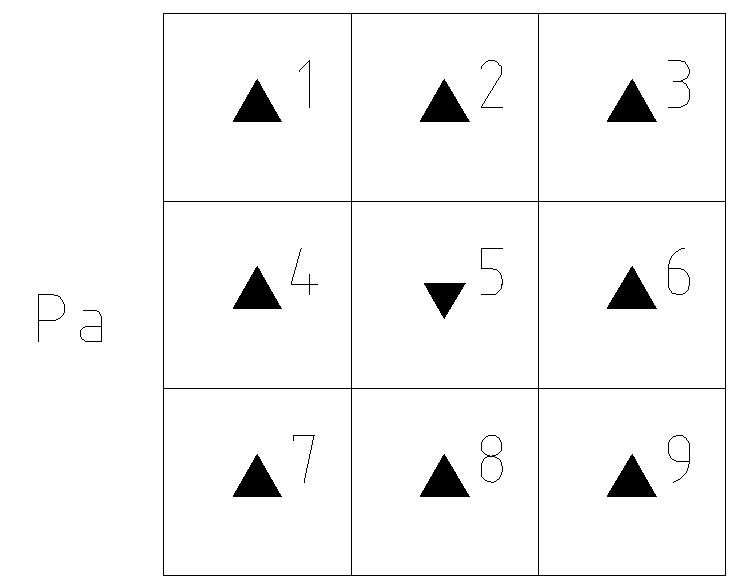
\includegraphics[width=14pc]{1.png}}
	\caption{Схема расчётной области]}
	\label{fig:map}
\end{figure}

	\section{Пятиточка}
\begin{figure}
	\center{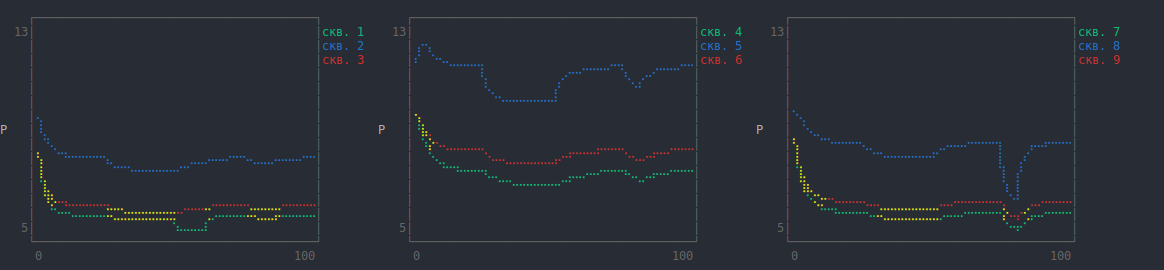
\includegraphics[width=30pc]{2.png}}
	\caption{Пластовое давление по скважинам}
	\label{fig:map}
\end{figure}
\begin{figure}
	\center{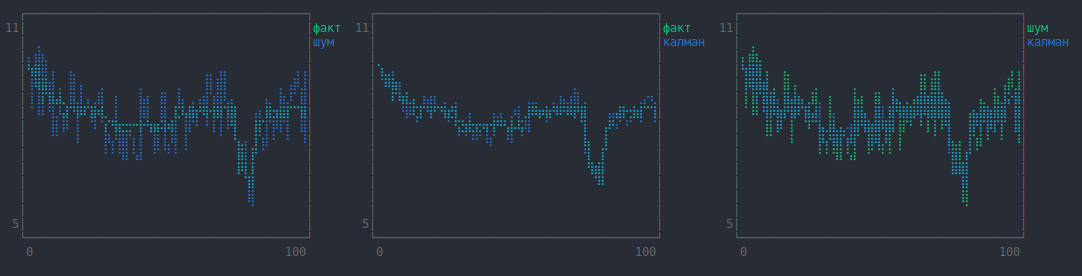
\includegraphics[width=30pc]{3_8.png}}
	\caption{Пластовое давление по скважинам}
	\label{fig:map}
\end{figure}
\begin{figure}
%	\center{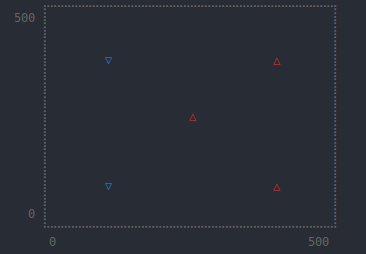
\includegraphics[width=14pc]{best_5well.png}}
%	\caption{Наилучшая схема назначения скважин]}
%	\label{fig:map}
\end{figure}
\begin{figure}
%	\center{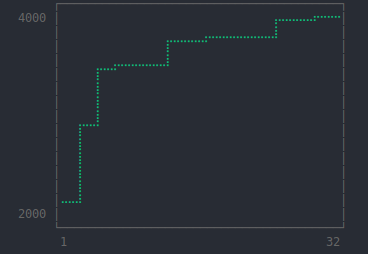
\includegraphics[width=14pc]{JJ5well.png}}
%	\caption{Схема расположения скважин]}
%	\label{fig:map}
\end{figure}

	\section{Девятиточка}
	\begin{figure}
%		\center{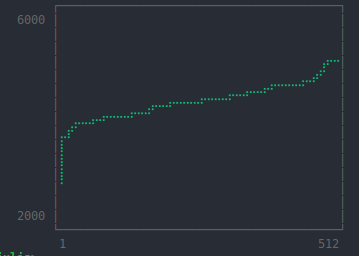
\includegraphics[width=24pc]{JJ9well.png}}
%		\caption{Значение ЦФ полный перебор]}
%		\label{fig:map1}
	\end{figure}
	\begin{figure}
%		\center{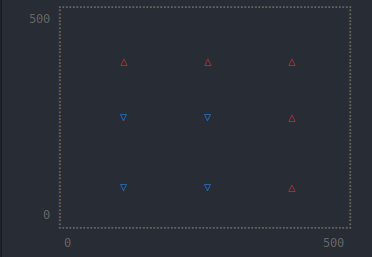
\includegraphics[width=24pc]{best_9well.png}}
%		\caption{Наилучшая схема назначения скважин]}
%		\label{fig:map2}
	\end{figure}
	\begin{figure}
%		\center{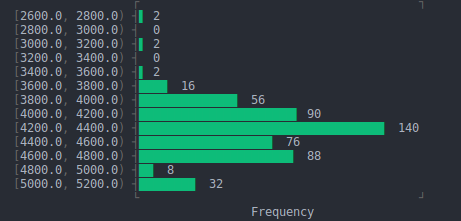
\includegraphics[width=24pc]{hist_JJ9well.png}}
%		\caption{Схема расположения скважин]}
%		\label{fig:map3}
	\end{figure}
	\begin{figure}
%		\center{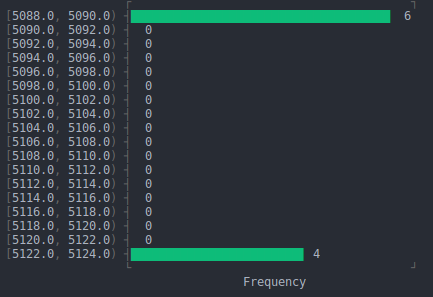
\includegraphics[width=24pc]{hist_JJ9well_alg.png}}
%		\caption{Схема расположения скважин]}
%		\label{fig:map4}
	\end{figure}

\end{document}